% For a masters thesis, replace the above \documentclass line with
% \documentclass[masters]{ucbthesis}
% This affects the title and approval pages, which by default calls this
% document a "dissertation", not a "thesis".

\documentclass[masters]{ucbthesis}

% support display of graphics
\usepackage{graphicx}

% import library of technical symbols
\usepackage{amsmath,amssymb,latexsym}

% import bibliography tools
\usepackage{natbib}
\citestyle{aa}

% To compile this file, run "latex thesis", then "biber thesis"
% (or "bibtex thesis", if the output from latex asks for that instead),
% and then "latex thesis" (without the quotes in each case).

% Double spacing, if you want it.  Do not use for the final copy.
% \def\dsp{\def\baselinestretch{2.0}\large\normalsize}
% \dsp

% If the Grad. Division insists that the first paragraph of a section
% be indented (like the others), then include this line:
% \usepackage{indentfirst}

\begin{document}

% Declarations for Front Matter

\title{HYPERION: The Case for Interferometry in 21 cm Reionization Global 
Signal Studies}
\author{Kara Kundert}
\degreesemester{Fall}
\degreeyear{2018}
\degree{Master of Astrophysics}
\chair{Professor Aaron Parsons}
\othermembers{Professor Martin White \\
  Professor Eugene Chiang}
\numberofmembers{3}
\field{Astronomy}
\campus{Berkeley}

\maketitle
% Delete (or comment out) the \approvalpage line for the final version.
\approvalpage
\copyrightpage

% (This file is included by thesis.tex; you do not latex it by itself.)

\begin{abstract}

% The text of the abstract goes here.  If you need to use a \section
% command you will need to use \section*, \subsection*, etc. so that
% you don't get any numbering.  You probably won't be using any of
% these commands in the abstract anyway.

In this memo, we seek to lay out a case for the use of absorber in an 
 interferometric study of the spatial monopole of the 21cm reionization 
 signature (i.e. the ``global signal"). As discussed in previous memos, we 
 believe that the way to optimize the sensitivity to the monopole term comes 
 from the use of absorptive walls between the antennas to impose an 
 artificially high ``horizon", or temperature discontinuity, onto the beam of 
 each antenna, thereby pushing the monopole into higher order spatial 
 terms~\citep{kundert2016}. With the new simulation, we are able to manipulate 
 many parameters of our virtual interferometer, including but not limited to 
 the antenna spacing, absorber wall height, and the attenuating properties of 
 the absorber itself.  From our exploration of these parameters, we are able to 
 now state with certainty that we are able to detect the monopole term of the 
 sky using a classical interferometer.

\end{abstract}


\begin{frontmatter}

\begin{dedication}
\null\vfil
\begin{center}
 \noindent{\large{\emph{Failure is simply the opportunity to begin again,\\ 
 this time more intelligently.}}\\ \normalsize{-- Henry Ford}}
\end{center}
\vfil\null
\end{dedication}

% You can delete the \clearpage lines if you don't want these to start on
% separate pages.

\tableofcontents
\clearpage
\listoffigures
\clearpage
%\listoftables

\begin{acknowledgements}
 This work would not have been possible without the financial support of the 
 National Science Foundation CAREER Award, the International House Carl \& 
 Betty Helmholz Gateway Fellowship, or the University of California, Berkeley 
 Department of Astronomy. 

 I must also give ample thanks to those with whom I have had the pleasure of 
 working on this and related projects. In particular, I would like to thank 
 Cherie Day, who has given me her love, her support, and her valuable 
 scientific and engineering insights since my first day on the Berkeley campus.  
 I would also like to thank the past and present members of the HYPERION team, 
 including Nipanjana Patra, Sanah Bhimani, Trisha Bhattacharya, Daniel Shen, 
 Raj Biswas, and Liju Phillip. Their hard work, patience, and, at times, upper 
 body strength, have made this project what it is today.  I could not have 
 reached this point without their combined abilities, and I am endlessly 
 grateful for their contributions.

 I would also like to thank the various members of the department who have 
 helped me along the path to completing this thesis. To Fatima Abdurrahman, 
 thank you for the dumplings and your friendship. To Charles Goullaud, thank 
 you for letting me unload my stress over some of your very fine whiskey and 
 some very silly movies. To Deepthi Gorthi, thank you for walking with me when 
 I needed to get out of the department and get some perspective. To Tom Zick, 
 Carina Cheng, and Zaki Ali, thank you for stepping in and providing me with 
 support when I most needed it.

 I am so grateful to my friends outside of the department, who have been 
 endlessly and creatively supportive along this journey. To Tristan Scroggins, 
 thank you for believing in me when I did not. To Adham El-Batal, thank you for 
 always understanding me and always knowing the right thing to say. To Tj 
 Carskadon, thank you for always being there for me, no matter whether I need 
 career advice, a study buddy, a drinking partner, a pep talk, or a hug.  To 
 Cameron Chalker, thank you for not listening to my excuses and always driving 
 me to give my best, and for reminding me of the consequences of reneging on 
 our long-standing deal.

 Finally, I cannot adequately express how grateful I am to my father. He has 
 always been my greatest ally and continues to support me in every way he can. 
 I would not have been able to complete this thesis without him standing 
 steadfastly in my corner.

\end{acknowledgements}

\end{frontmatter}

\pagestyle{headings}

\chapter{The Global Signal -- Its Physics and Significance to Cosmology}

\section{Overview of the Epoch of Reionization}

In brief, the Epoch of Reionization refers to the period of the universe's 
history during which its supply of intergalactic hydrogen became reionized.  
This is important to its evolution, and therefore of interest to astronomers, 
due to the driving factor of that ionization: the ignition of the first stars, 
galaxies, and black holes in the universe. A positive detection of the Epoch of 
Reionization will help astronomers to clarify many open questions of cosmology, 
such as the properties of the first galaxies, how stars with zero metallicity 
formed, the physics of early quasars, and more.

In slightly more detail, let us begin at the beginning. At the start of time, 
the universe was extremely hot and ionized from the Big Bang. Over time, as 
space itself expanded and the gas within the universe cooled adiabatically 
along with that expansion, the temperature of the universe dropped low enough 
that the nearly uniform ionized plasma that made up the universe was able to 
recombine to form neutral hydrogen. This phase transition, which occurred 
approximately 400,000 years after the Big Bang, enabled photons to decouple 
from the baryonic matter, allowing photons to stream freely for the first time 
in the history of the universe.  Those photons are what we now know as the 
``Cosmic Microwave Background" (CMB).

At the point of the CMB, the gravitational force had heretofore always served 
as second fiddle to the electromagnetic force, and the formation of structure 
was driven solely by dark matter~\citep{zaroubi2012}.  As such, structure had 
yet to form, and the release of the CMB led to a period known as the ``Dark 
Ages" -- a time when the universe had nothing to do but slowly get to work 
allowing slight matter over-densities grow and transform into stars, galaxies, 
and black holes.

So, about 100 million years passed and the universe bathed in nothing but the 
after-glow of the Big Bang. Finally, the first galaxies formed, and along with 
them bright stars to emit ionizing radiation. Soon, we find small ionized 
bubbles in the intergalactic medium (IGM), the hydrogen gas filling the space 
between galaxies. Over time, more galaxies and their bright stars make more 
ionized bubbles, until eventually the entire universe's supply of loose 
hydrogen gas has been converted into a proton-electron ionized plasma.

This period, very creatively, is called the Epoch of Reionization -- the epoch 
during which the universe once again became ionized, like it was at the dawn of 
time.

As of yet, there has been no confirmed direct detection of this time period -- 
either of the objects that drive it nor of the gas behavior itself. This is not 
for lack of trying. There are currently (or soon to be) observatories looking 
for high-redshift galaxies and quasars~\citep{gardner2006}, for power-spectrum 
measurements to find ionized regions around those high-energy 
objects~\citep{deboer2017}, and for the microscopic temperature changes in the 
gas of the universe~\citep{bowman2018}.  As it turns out, these observations 
are hard to make -- 13 billion light years is a long way for light to travel.

For the sake of brevity and intellectual focus, this thesis (and the experiment 
proposed within) will be focusing solely on observing the overall average 
behavior of the intergalactic medium as it evolves throughout this time period.  
This is referred to as the ``global signal".

\section{Overview of the Global Signal}

The global signal of reionization is an observation of the overall average 
nature of hydrogen throughout this epoch, i.e. the spatially averaged signal 
from the neutral hydrogen gas, as observed using redshifted 21 cm emission from 
the intergalactic medium 13 billion years ago. More specifically, global signal 
experiments seek to observe the relationship between the gas temperature and 
the ambient temperature of the universe, as set by the CMB photons.  By 
observing the evolution of the thermal gas temperature ($T_K$) relative to the 
photon temperature ($T_\gamma$), we are able to better understand how and when 
energy was injected into the gas~\citep{pritchard-loeb2010}. For example, the 
X-rays generated by black holes contributed to the heating of the gas, making 
the gas itself brighter than the ambient photons. Additionally, Lyman-$\alpha$ 
photons from Population II and III stars modify the coupling of the IGM gas 
temperature to the 21 cm spin temperature via the Wouthuysen-Field effect, 
providing a means to track early star formation~\citep{furlanetto2006}.

This signal ($T_b$) is measured as a function of four main variables -- the 
thermal temperature of the hydrogen gas ($T_K$), the volume-averaged ionized 
fraction of hydrogen ($x_i$), the specific flux of the Lyman-$\alpha$ frequency 
($J_\alpha$), and the number density of hydrogen ($n_H$). One particularly 
convenient aspect of $T_b$ is that its dependence on each of these quantities 
saturates at some point, leading to clear and separate regimes in the history 
of the signal that can only be described by the changes in one 
variable~\citep{pritchard-loeb2012}. These regimes can be seen in 
Fig.~\ref{fig:global-signal}, and are physically detailed below.

\begin{figure}
    \begin{center}
    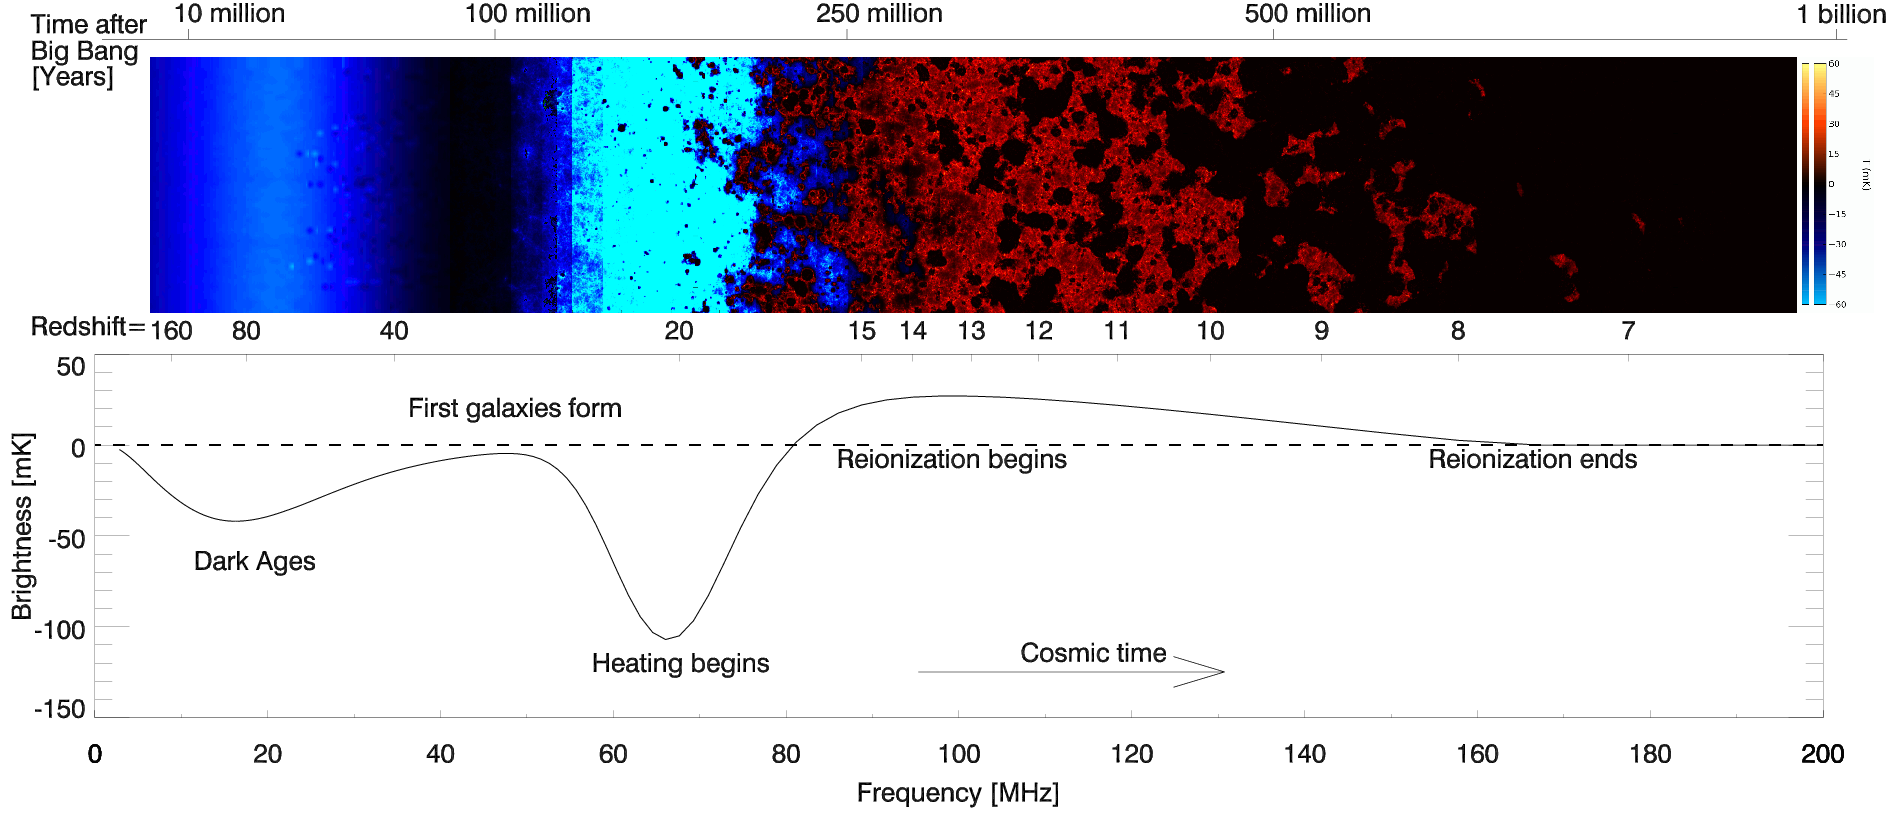
\includegraphics[width=\linewidth]{global_signal.png}
    \end{center}
    \caption{
        In the top half of the figure, we see a cartoon of the reionization 
        history of the universe and the development and growth of ionized 
        bubbles over time. In the bottom half, we see a breakdown of $T_b$, the 
        brightness temperature of the 21 cm global signal, over time. There are 
        five labeled regimes to this plot, each corresponding to the dominance 
        of a different variable in the production of the 21 cm signal. Figure 
        originally published in~\citealp{pritchard-loeb2012}.
    }
    \label{fig:global-signal}
\end{figure}

\subsection{Brief History of the Global Signal}
\begin{itemize}
    \item[--] (200 $\leq z \leq$ 1100): During this time period, the residual 
     free electron fraction remaining post-recombination and the high gas 
     density allows the thermal and spin temperatures of the gas to remain 
     coupled with the photon background via Compton scatting and collisional 
     excitations. All temperatures are the same, and therefore there will be no 
     detectable 21 cm signal.
    \item[--] (40 $\leq z \leq$ 200): As cosmological expansion continues, 
     Compton scattering no longer couples the thermal temperature of the gas to 
     the CMB photons, and the gas and radiation decouple and go out of 
     equilibrium.  Collisional coupling sets the spin temperature $T_S < 
     T_\gamma$, leading to an absorption feature in the 21 cm global signal.  
    \item[--] (30 $\leq z \leq$ 40): Expansion continues and collisional 
     interactions are no longer effective at coupling the thermal and spin 
     temperatures of the gas. The excitation levels shift to being set by 
     radiative coupling to the CMB, such that $T_S = T_\gamma$, and there is no 
     detectable 21 cm signal.
    \item[--] (15 $\leq z \leq$ 30): As the first sources (e.g. stars, active 
     galactic nuclei (AGN), etc...) ignite, they begin emitting high energy 
     Lyman-$\alpha$ and X-ray photons. The hyperfine populations couple to the 
     thermal temperature of the cold gas via the Wouthuysen-Field effect, such 
     that $T_S \sim T_K < T_\gamma$, resulting in an absorption feature in the 
     21 cm global signal.
    \item[--] (7 $\leq z \leq$ 15): The radiation (particularly the X-rays) 
     from bright sources heat the gas, $T_K > T_\gamma$ and we see 21 cm 
     emission in the global signal. Lyman-$\alpha$ coupling is still effective 
     at setting the level populations.
    \item[--] ($z \leq$ 7): Enough ionizing radiation has spread throughout the 
     universe that the IGM has been converted from neutral to ionized, and 
     reionization is complete.
\end{itemize}


\chapter{CHAPTER TITLE}

\section{Results}

lay out the case that absorber helps us maximize interferometric sensitivity to 
monopole, lay out the case that we can use the characteristics of this 
sensitivity to potentially help us pick out monopole vs. higher order terms 
(some kind of filtering around sensitivity vs. u mode)

\begin{figure}
    \begin{center}
    \includegraphics[width=\linewidth]{/home/kara/documents/hyperion/memos/flat_sky_no_abs_freq.png}
    \end{center}
    \caption{
        Shown here is the absolute value of the visibility of a spectrally flat 
        monopole sky with no absorber walls versus frequency. As can be seen 
        already, the interferometer does have non-zero sensitivity to the 
        monopole, though it is plainly clear that the autocorrelation term 
        (i.e. Baseline 0) is more sensitive than any of the non-zero 
        interferometric baseline pairings listed in Table~\ref{tab:baselines}.
    }
    \label{fig:flat-sky-no-abs-freq}
\end{figure}

\begin{figure}
    \begin{center}
    \includegraphics[width=\linewidth]{/home/kara/documents/hyperion/memos/flat_sky_no_abs_uv.png}
    \end{center}
    \caption{
        Shown here is the absolute value of the visibility of a spectrally flat 
        monopole sky with no absorber walls versus uv-baseline. As can be seen 
        already, the interferometer has a non-zero sensitivity to the monopole 
        at non-zero baseline separations.
    }
    \label{fig:flat-sky-no-abs-uv}
\end{figure}

\chapter{Overview of the Theory of HYPERION}

\section{Absorber -- A New Approach to Monopole Interferometry}

If you were to wander onto almost any given radio telescope currently active in 
taking observations, you're almost certain to find some kind of reflective 
material underneath the antennas (either in the form of a ground screen or a 
reflective dish). One thing you're not likely to find is any kind of absorptive 
material -- we as astronomers are already fighting an uphill battle on 
attaining the very fine sensitivities needed to detect celestial sources, we 
really need all the photons we can get. 

However, it is not unheard of. While absorbers have never been used in the 
element design of a reionization project to date, they have been used by cosmic 
microwave background (CMB) experiments. Absorptive structures, or baffles, to 
control pickup from outside the main beam, which can be a source of systemic 
errors~\citet{essinger-hileman2016}. By surrounding the receiver with an 
absorptive material, rather an a reflective one as seen in most standard radio 
telescope designs, one can better control the exact signal that will be seen in 
the sidelobes of the beam, and thereby better calibrate the system in turn.

This same principle applies in the case of a monopole interferometer, where use 
of an absorber can not only be beneficial but actually fundamental to the 
design of the array despite the microscopic signal we aim to detect. By 
controlling what each antenna sees on the sky, we can accurately calibrate our 
system and ensure that our reionization signal is indeed signal and not 
instrumental noise. 

\subsection{Practical Instrumentation}

As discussed in Chapter~\ref{chap:interferometry}, one of the fundamental 
requirements of a monopole interferometer is close spacing of the antennas, in 
order to maximize reception of the global sky mode. However, this close spacing 
also predisposes the instrument to cross-talk. As discussed 
in~\citet{venumadhav2016}, this isn't necessarily a bad thing -- cross-talk is 
one of two ways that an array of antennas can maintain a sensitivity to the 
monopole. Each individual antenna will broadcast its reception of the monopole 
to its neighbors, and that reception will correlate. In this case, one will 
have a direct view of the monopole term, as you will be correlating the 
zero-spacing mode seen by one antenna with the zero-spacing mode of another, 
thus providing the necessary sensitivity to the global signal. 

However, that also means that instrumental noise will be broadcast and 
correlated between antennas, vastly diminishing the useful properties of the 
interferometer and maintaining many of the pitfalls of single-dish instruments.  
The risk here comes in the calculus of calibration for the instrument.
In particular, it is difficult to properly calibrate the correlated noise 
between elements as it has a noise bias. This bias means that, while we observe 
more of the true signal, we also no longer are able to integrate down the 
instrumental noise, essentially placing a DC offset into our system. The exact 
value of this offset is a function of frequency and of the exact qualities of 
the instrument, and will likely vary from element to element. If it is not 
perfectly calibrated and subtracted off from the data, then traces of this bias 
will remain in the final data and can easily be mistaken for true science.

So we'd like to avoid cross-talk and other sources of correlated noise between 
elements as best as we can, while still maintaining a sensitivity to a 
correlated monopole signal. The only other way for an interferometer to have 
the capacity to observe the monopole is through the presence of dissipative 
elements, such as absorbers and/or the ground.  Without cross-talk or 
dissipative elements, the monopole term will integrate to zero in every 
non-zero spatial mode, making the interferometer completely insensitive to the 
global signal~\citet{venumadhav2016}.

One way to manage cross-talk it to pack the space between antennas with 
absorber -- with a high-enough quality absorber, we can essentially make the 
antennas invisible to each other by just placing a tall enough wall between 
them.  Ideally, this material would be quite physically thin, so that these 
absorber walls wouldn't force us to spread the shape of the array at all, thus 
maintaining a sensitivity to the spatial monopole of the reionization global 
signal.

In order for this to work, the absorber needs to meet some basic criteria. Most 
importantly, it will need to be at least optically thick enough that antennas 
on opposing sides of an absorber wall will not observe the same noise signal 
from the absorber. If the noise observed from the absorber is coherent between 
elements, then we will fall into the same pitfalls that arise from cross-talk 
between elements, described above.

Additionally, the absorber walls need to be shaped in such a way that signal 
won't reflect and bounce over the barriers -- if signals are able to diffract 
off of one antenna and into the other, then there will still be cross-talk and 
our calibrations will be flawed. For this reason, we won't be able to build 
straight walls with sharp cutoffs. Rather, we want to build our walls in a way 
that signal gets trapped into the absorber or angles out of the array entirely.  
Ideally, we'd like to build our walls with some kind of pyramidal structure (to 
capture and dampen the signal within the absorber), and with a curved roll-off 
at the top edge (to prevent reflections off of the baffle into multiple 
antennas).

\subsection{Manipulating the Spatial Monopole}

Another benefit to the use of absorber in our array is how we can use it to 
manipulate the instrument's sensitivity to the monopole.  As discussed in 
Sec.~\ref{sec:observing-monopole}, by applying a spatial windowing function to 
our monopole signal, we can increase our interferometric sensitivity to the 
global signal. The absorber can impose this windowing function by creating a 
spatial temperature change in the absorber's field of view, increasing the 
harmonic content of the monopole signal by imposing non-isotropic terms.

\begin{figure}
    \begin{center}
    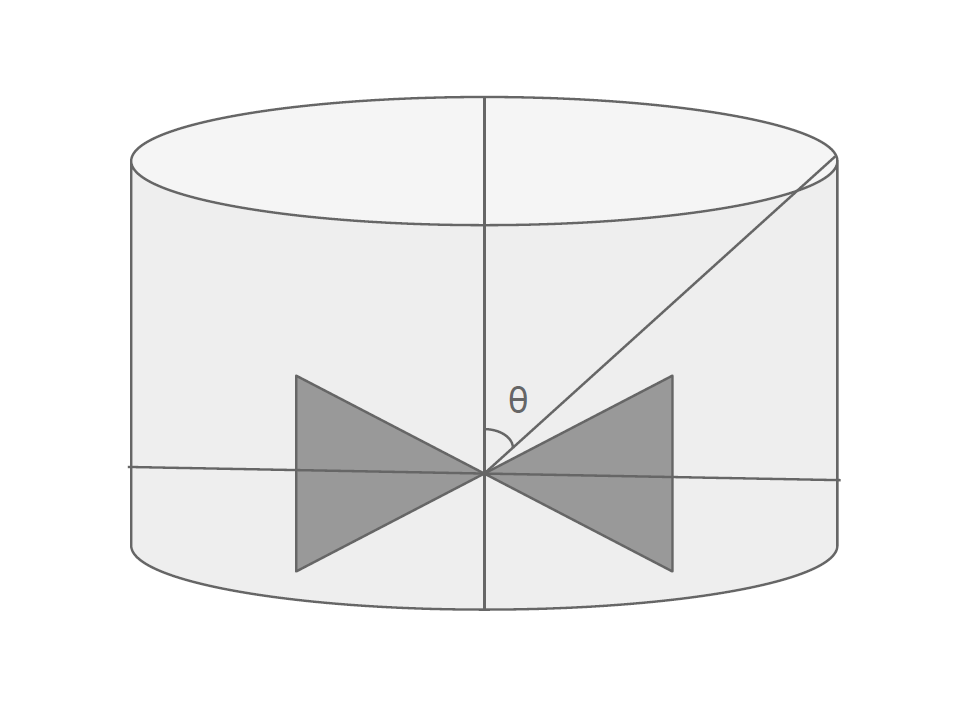
\includegraphics[width=\linewidth]{absorber-structure.png}
    \end{center}
    \caption{
        This cartoon shows the basic structure of the proposed absorber walls.  
        Each antenna in the array will be circled by a cylinder of absorber 
        material, creating a uniform temperature cutoff in the antenna's 
        reception of the sky. By increasing the height of the wall, we can 
        change the cutoff angle of the reception of the sky, thereby shrinking 
        the spatial windowing and pushing more of the monopole to higher 
        spatial modes.
    }
    \label{fig:absorber-structure}
\end{figure}

Let's take a closer look at how this is to actually work. In a perfect world, 
our absorbing material would be $100\%$ effective and no information could be 
transmitted through it -- it would absorb all incident light and re-emit it as 
thermal radiation. That means that, as per Fig.~\ref{fig:absorber-structure} 
and ignoring the effects of the antenna beam shape, the antenna would see the 
sky up until an angle of $\theta$ off of zenith, and then it would see a 
perfect blackbody matching the ambient temperature of the array everywhere 
else.

One way to understand the absorption of the blackbody would be to think in 
terms of optical depth, and the above case is one in which the absorber has an 
optical depth of $\tau = \infty$. This thinking also enables us to begin to 
understand more realistic scenarios, where we don't have perfect absorption 
between our antennas.

\begin{equation}
    I_{obs}(\theta) = I_{sky}~e^{-\tau_\theta} + S_{abs}~(1 - e^{-\tau_\theta})
    \label{eq:abs-optical-depth}
\end{equation}

where $I_{obs}$ is the observed sky brightness, $I_{sky}$ is the sky 
brightness, $S_{abs}$ is the thermal brightness from the absorber, and $\tau$ 
is the optical depth of the absorber. This equation is a variation on the 
radiative transfer equation, where the sky is our source and the absorber is 
the medium through which the radiation is travelling.

In this quantitative construction of the reception of an element, we can see 
that the strength of the absorber determines the strength of the spatial cutoff 
-- particularly, in the case of a poor absorber, the above equation shows that 
there will be a great deal of sky leakage into the ``horizon". In particular, 
for reionization studies, this will be problematic due to the brightness of the 
sky at these frequencies from galactic synchrotron emission. So a weak absorber 
will barely put a dent in the sky brightness, diminishing the effectiveness of 
the imposed window, and keeping the reionization global signal power in the 
lower, harder to detect spatial modes.

Additionally, if the quality of the absorber is poor, this can increase the 
confusion between inherent sky structure and windowed monopole sky. Consider 
the fact that the sky itself will not be a perfect monopole and will therefore 
have spatial structure. If the quality of the absorber is poor, then more of 
that structure will be visible across the whole sky. This will exist in 
addition to the characteristic spatial sensitivity of the monopole portion of 
the sky. This mixing of intrinsic sky structure and imposed sky structure must 
be handled carefully, and having a high-performing absorber can help us to 
better control those parameters.

Finally, if the absorber is optically thin, then antennas on either side of an 
absorber baffle will see coherent signal coming from the absorber, contributing 
to an overall noise bias that may be hard to calibrate for.

\section{Overview of the Instrumental Design}

Let us now consider the design of our interferometer itself. There are two key 
areas of interest to us: how our sensitivity to the monopole varies with the 
separation between antennas, and how it changes in the presence of different 
absorber structures and materials. Another way of viewing it would be: how do 
the characteristics of the individual elements and of the array design affect 
our ability to make this measurement.

Let us first consider the array design, i.e. baseline separations. Intuitively, 
we expect that the sensitivity to the global signal will be maximized with the 
smallest baseline separations, which correspond to a position in the 
\emph{uv}-plane close to the origin, or the zero-spacing mode.  The trade-off 
of this, from a design perspective, comes in the difficulty of ameliorating 
cross-talk in a densely packed array. We want to optimize our array design to 
space our antennas as loosely as possible while also maintaining workable 
sensitivity to the monopole term, as this will best enable us to mitigate 
systemic problems in our instrument and perform a successful experiment.

The next step is to add the absorber, which can essentially be treated as a 
modification to the antenna's beam. This calculation is done using 
Eq.~\eqref{eq:absorber-baffle},

\begin{equation}
    \label{eq:absorber-baffle}
    B(\theta, \phi, \nu) = 10^{\alpha(\nu)/20} \Big(\frac{1}{2} + \frac{1}{2} 
    \tanh\Big(\frac{\theta - (\frac{1}{2} - \theta_{0})}{a}\Big)\Big) +
    \Big(\frac{1}{2} - \frac{1}{2} \tanh\Big(\frac{\theta - (\frac{1}{2} - 
    \theta_{0})}{a}\Big)\Big)
\end{equation}

where $\alpha(\nu)$ is the absorptivity by frequency of the absorber, 
$\theta_0$ is the cutoff angle of the structure (i.e. $\theta_0$ is the height 
of the absorber walls), and $a$ is the smoothing parameter that blends the 
transition between the absorber and the sky.

This term is then combined with the antenna beam, giving us 
Eq.~\eqref{eq:absorber-beam}.

\begin{equation}
    \label{eq:absorber-beam}
    A'(\theta, \phi, \nu) = A(\theta, \phi, \nu) B(\theta, \phi, \nu)
\end{equation}

One thing to note about our particular experiment is that there is no need for 
cryogenic cooling. As mentioned in Section~\ref{sec:eor-overview}, the expected 
values for the 21 cm reionization global signal are far, far fainter than that 
of the ambient emission from our own galaxy. In the proposed science band for 
HYPERION, we expect the galactic synchrotron component of the sky brightness 
temperature to range from about 650--3700 K~\citep{haslam1982}. This is, at 
best, 40,000 times brighter than the reionization signal that we are seeking.

This also means that there is no need to cool the absorber baffles -- the sky 
is bright enough on its own to easily dominate the overall system temperature, 
so leaving the absorbers warm has no significant effect~\citep{kundert2016},

\chapter{Overview of the Logistics of HYPERION}

\section{Methodology of Simulation}

For this simulation, we import a model array using the AIPy AntennaArray 
framework, which enables us to carry around an array with known geometry and 
baseline separations, along with individual antenna beam patterns and 
accessible frequencies. With this information and the previously made sky maps, 
we are now able to calculate our visibilities across many frequencies by using 
Eq.~\eqref{eq:vis}.

The AntennaArray framework also enables us to carry around models of the beams 
of the antennas, which is a convenient way to import absorbers into the 
simulation. Essentially, within the context of the simulation, the absorbers 
act as a modification term on the beam pattern, changing the way that each 
individual antenna sees the sky. This works as follows:

To start, we need a beam. HYPERION uses SARAS-style fat dipole antennas in our 
instrument, which means we will be using a frequency-invariant dipole beam 
pattern in our simulation to match~\citep{patra2013}. This is the base beam 
model used throughout the simulation, calculated using 
Eq.~\eqref{eq:dipole-beam}.

\begin{equation}
    \label{eq:dipole-beam}
    A(\theta, \phi, \nu) = \cos\Big(\frac{\frac{\pi}{2} 
    \cos{\theta}}{\sin{\theta}}\Big)
\end{equation}

The parameters we can play with are the absorptivity of the material (i.e. how 
much attenuation does the absorber provide at each frequency), the height of 
the absorber walls, and how smooth the transition from absorber to sky is.  

\section{Absorber Baffles -- Initial Results}

TALK ABOUT SYSTEM TEMPERATURE, NO NEED TO COOL BAFFLES (memo 1)

To date, we are still relatively early in the testing of our hypothesis that 
absorber walls or ``baffles" between antennas will enable us to better observe 
the spatial monopole with an interferometer. There have been two main sets of 
tests performed so far -- one in-lab test to measure the absorptivity of 
various proposed materials, and some brief field tests to gauge the 
effectiveness of our absorber at mitigating cross-talk between antennas.

The in-lab test was, in essence, a simple antenna return-loss measurement. To 
conduct the measurements, we started by constructing a large (i.e. 4.5' cube) 
Faraday cage out of wood and chicken wire, and placed an antenna at its center.  
From this setup, we could perform a simple return loss measurement and see what 
the maximum power return to the antenna is.

We could then line the cage with various absorptive materials and take another 
return-loss measurement, this time with (ideally) much of the power absorbed by 
the absorber, and see how effective each material is at dissipating energy 
within our science band. One such measurement is shown in 
Fig.~\ref{fig:fe-absorption}, featuring our most promising absorber candidate 
material, ferrite tiles.

\begin{figure}
    \begin{center}
    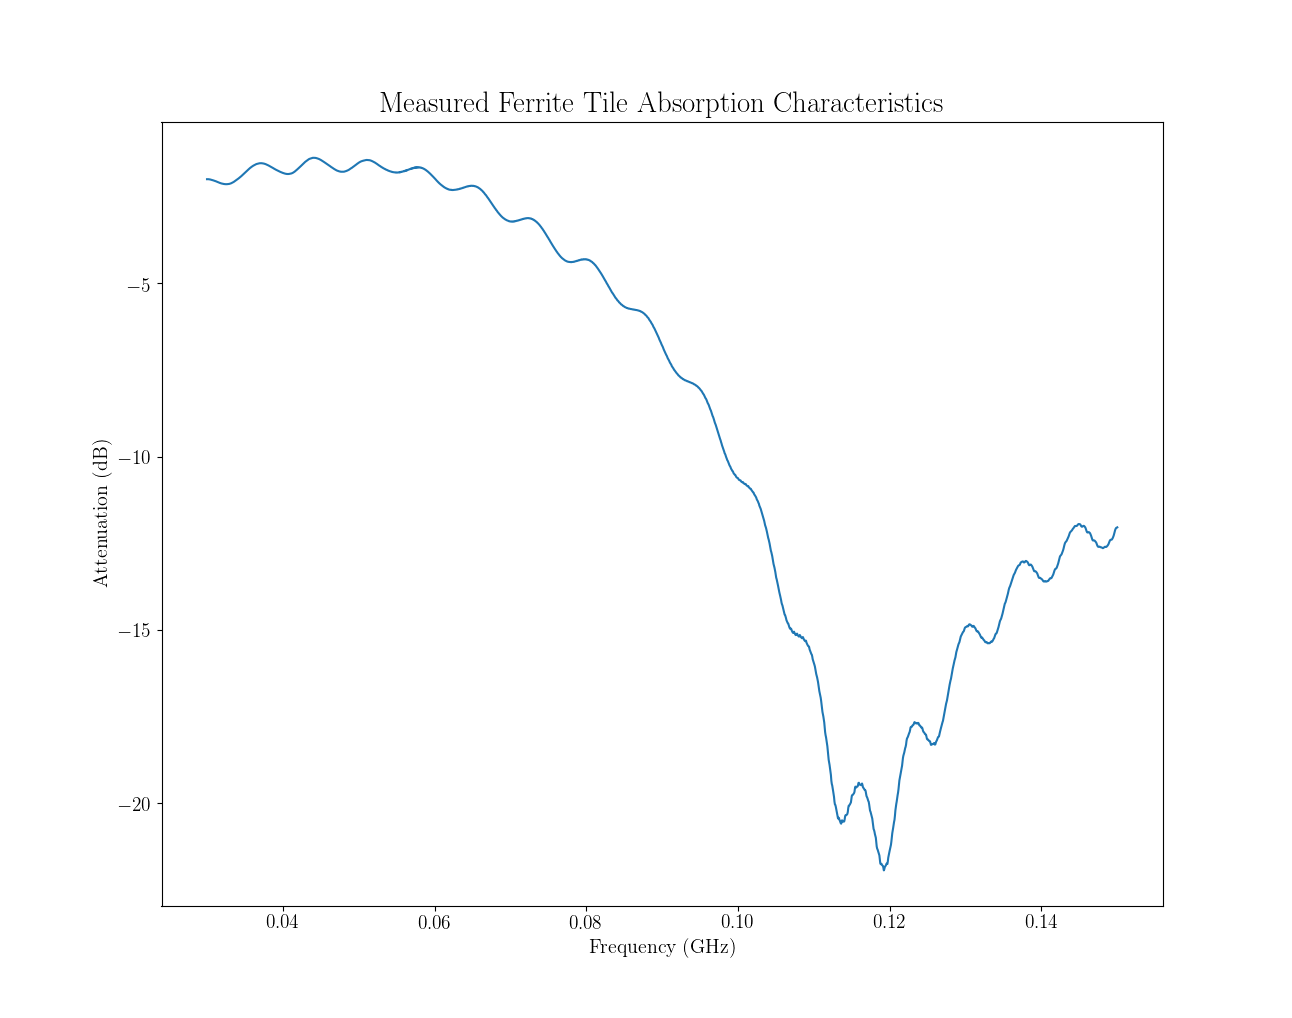
\includegraphics[width=\linewidth]{fe_absorption.png}
    \end{center}
    \caption{
        Here we see the results of a closed-box return loss measurement taken 
        with a densely packed (i.e. $9\times9$ tiles per wall) configuration of 
        ferrite tiles, evenly spaced along the walls of the testing Faraday 
        cage. The ripples are an artifact from the testing setup, and not 
        inherent to the performance of the ferrite itself. As can be easily 
        seen, the Ferrite performs much better at the high range of our science 
        band, and is optimized around $\sim120$ MHz.  While this material has 
        the best performance out of all the materials we have looked into so 
        far, we would ideally prefer a material with a more even absorptivity 
        across the band, so as best to avoid inadvertently adding ripples or 
        structure to our sky observations.
    }
    \label{fig:fe-absorption}
\end{figure}

As can be easily seen in the figure, the ferrite tiles have a decent 
absorptivity profile across the band, and an excellent absorptivity around 120 
MHz. However, as described in Section~\ref{sec:global-signal-overview}, the 
global signal of reionization is rich with physical information that is 
uniquely tied to its changing amplitude by frequency. The kinds of variations 
that we see in the absorptivity across the band are dangerous for the 
well-being of our experiment, as they could translate to tricky or uncertain 
calibration of our final instrument. We want to ensure that almost everything 
beyond the global signal has simple and well-defined relations to frequency 
(e.g. the synchrotron galactic sky, which is well described by a power law), in 
order to best understand our signal and be sure that instrumental 
idiosyncracies aren't being mistaken for true signal and science. As such, we 
would strongly prefer an absorber (or combination of absorbers) that has a more 
uniform performance across the science band.

Additionally, the ferrite tiles are among the most expensive of the materials 
we investigated. Even with a very close spacing and therefore relatively small 
baffle structures, the costs of acquiring enough ferrite to create an array 
quickly becomes overwhelming to the budget.
%\footnote{Of course, there's no longer any need to worry about that because 
%there is no budget -- this project dies alongside my academic ideals.}.

Other candidate absorbers include mats of Zotefoam Plastazote\textregistered, 
the AEP-EM low-frequency pyramidal foam absorber from DJM Electronics, and the 
creation of a grid of resistors designed to match with the free-space 
impedance~\citep{mahesh2015}. The Zotefoam was appealing due to its low cost 
compared to the pyramidal foam and ferrite tiles, but unfortunately its 
performance seemed to scale in proportion to its price tag.  The pyramidal foam 
performed slightly better, but seemed to feature more reflections than the 
ferrite and overall had a lower absorptivity performance than the ferrite, 
despite a nearly identical price tag per square foot of coverage. The resistive 
mesh is still an attractive idea, as it would only cost us an ungodly amount of 
effort to put together and about \$10 worth of resistors. Unfortunately, at the 
time of writing, only a very introductory level of investigation has been put 
into the resistive mesh idea, so nothing conclusive can be said about its 
performance as an absorber material.

At this point in time, there really haven't been any meaningful field tests 
upon which I could report. However, the most important things for us to 
investigate in the field would be a) ability of the absorber to mitigate the 
cross-talk between antennas and b) the efficacy of the baffles' ability to 
impose a spatial temperature variation from the antenna's point-of-view and how 
that efficacy evolves over frequency.

In Fig.~\ref{fig:field-test}, we see one possible arrangement of the absorber 
materials in order to assess the ability of the absorber at mitigating 
cross-talk between antennas. In order to perform this test adequately, one 
would need to take two measurements in the same radio environment -- one 
without the absorber between the antennas, in order to gauge the baseline level 
of cross-talk, and one with the absorber between, to measure the improvement in 
power leakage.

\begin{figure}
    \begin{center}
    \includegraphics[width=\linewidth]{field-test.png}
    \end{center}
    \caption{
        Shown here is a simple diagnostic field set-up that could be used to 
        evaluate an absorber's ability to mitigate cross-talk between elements.  
        Here we used a densely-packed configuration of ferrite tiles that have 
        been propped up on some of our pyramidal foam absorber for additional 
        height.
    }
    \label{fig:field-test}
\end{figure}

\chapter{Sensitivity to the Monopole Sky}

Now all that remains is actually answering the question of whether or not this 
could work.  Can a traditional interferometer actually pick up a global sky 
signal?  Can we manipulate that sensitivity using the strategic placement of 
absorptive materials around our antennas? And finally, and most importantly, 
can we actually understand the signals that we are sensitive to in order to 
accurately interpret our data, thereby actually observing the global signal of 
reionization?

\section{Simulated Visibilities}

Fundamentally, we are simply trying to calculate the visibility to the sky with 
a specific array set-up. We can describe this mathematically using the 
interferometric framework developed in Eq.~\eqref{eq:vis-allsky}. For the 
specific case we are investigating of a monopole sky and with absorptive 
baffles modifying the antenna beam, we get Eq.~\eqref{eq:vis-global-signal}:

\begin{equation}
 V(\nu) = T_{global}(\nu) \int A(\mathbf{s}) e^{-\tau(\mathbf{s,\nu})} e^{-2\pi 
 i \nu \mathbf{b}\cdot\mathbf{s}/c} ~d\mathbf{s}
    \label{eq:vis-global-signal}
\end{equation}

where $T_global$ is the temperature of the monopole sky, $A(\mathbf{S})$ is the 
antenna beam, $e^{-\tau(\mathbf{s})}$ is the spatial absorptivity, which is a 
function of direction and frequency. Here we see that the monopole sky has a 
convenient quality in that its lack of spatial information allows us to pull it 
out in front of the integral as a constant factor.

For our array, we will be considering the following set of perfectly east-west 
baseline separations: $\mathbf{b} = [0, \lambda/2, \lambda, 3\lambda/2, 
2\lambda, 3\lambda, 4\lambda]$ for a $\lambda = 100 MHz$.

Let's start by investigating the first question. Is an interferometer sensitive 
to the monopole sky? As described in Chapter~\ref{chap:logistics}, this can be 
be simulated, we just have to set our parameters appropriately.

We can begin with a very simplified proof-of-concept case. We will construct an 
array with no absorbers and a flat terrestrial horizon. Additionally, we will 
have beams with perfect receptivity in all directions, and a sky temperature of 
exactly $T_{global} = 1.0$ K across our entire observational band. This will be 
our most basic unit test -- something with which to check our intuition against 
and prove that the idea behind HYPERION is sound.

As expected and  as can be easily seen in 
Figures~\ref{fig:flat-sky-no-abs-freq} and~\ref{fig:flat-sky-no-abs-uv}, all 
ground-based interferometers have a non-zero sensitivity to the monopole mode 
of the sky. Similarly, we also find that the further we stray from the 
zero-spacing mode (i.e. as the number of wavelengths of separations increases), 
sensitivity to the monopole also quickly evaporates.

\begin{figure}
    \begin{center}
    \includegraphics[width=\linewidth]{/home/kara/documents/hyperion/memos/flat_sky_no_abs_freq.png}
    \end{center}
    \caption{
        Shown here is the absolute value of the visibility of a spectrally flat 
        monopole sky versus frequency. In this case, there are no absorptive 
        baffles, just the terrestrial horizon. As can be seen already, the 
        interferometer does have non-zero sensitivity to the monopole, though 
        it is plainly clear that the autocorrelation term (shown in blue) is 
        more sensitive than any of the non-zero interferometric baseline 
        pairings.
    }
    \label{fig:flat-sky-no-abs-freq}
\end{figure}

\begin{figure}
    \begin{center}
    \includegraphics[width=\linewidth]{/home/kara/documents/hyperion/memos/flat_sky_no_abs_uv.png}
    \end{center}
    \caption{
        Shown here is the absolute value of the visibility of a spectrally flat 
        monopole sky with no absorber walls versus uv-baseline. As can be seen 
        already, the interferometer has a non-zero sensitivity to the monopole 
        at non-zero baseline separations.
    }
    \label{fig:flat-sky-no-abs-uv}
\end{figure}

But this simple unit test tells us much more than just the fact that HYPERION 
is feasible after all. We can also begin to see a characteristic shape of the 
sensitivity in the \emph{uv}-plane, with peaks and nulls placed at regular 
intervals in \emph{uv}-space. The predictability of this shape could allow us 
to use it as a calibration tool, if properly understood. In particular, it 
could be a valuable way to remove leakage from non-monopole terms into our 
signal. Given that this characteristic shape derives only from the monopole sky 
and the shape of the beam, we know that any observational deviations in this 
shape must come from the sky rather than the system. Therefore, it may be 
possible to use this information as a way to filter out non-monopole terms from 
the sky, thus ensuring that we won't mix up spectral wiggles from the 
combination of various non-monopole sky sources with our expected wiggly 
reionization global signal, as seen in Fig.~\ref{fig:global-signal}. Instead, 
we can, effectively, select just the monopole terms of the sky -- the galactic 
synchrotron background and the reionization global signal -- thus ensuring that 
the only terms we're left with have simple relationships with frequency that 
can be easily parsed from the frequency-independent evolution of the 
reionization term.

Additionally, this characteristic shape could enable  us to do some weighting 
of our observational data. By knowing exactly what modes we expect to see the 
monopole term at its brightest and dimmest, we could properly weight and 
interpret data at each mode and frequency, enabling us to better compare data 
points at different points in \emph{uv}-space and frequency.

So we have established that we can detect the monopole with an interferometer, 
which is step one. But, as we can see, that sensitivity is faint, especially at 
the high-frequency end of our science band. That by itself is not wholly 
problematic -- we could just run our observation longer and beat down our 
sensitivity, assuming we still keep our spacing close enough that our 
observations don't have to run infinitely long. What is problematic is the 
strong cross-talk between elements that we know we'll face when we place them 
that close. We need to make our elements invisible to each other, and we think 
we can simultaneously enhance our sensitivity to the monopole as well.

In our next set of tests, we include the absorptive baffles around each 
antenna, as described in previous chapters. Using the absorption profile of the 
ferrite tiles, as seen in Fig.~\ref{fig:fe-absorption}, we can see how the 
monopole sensitivity is changed in the presence of the baffles.

As can be seen in Figures~\ref{fig:flat-sky-fe-abs-freq} 
and~\ref{fig:flat-sky-fe-abs-uv}, the sensitivity of the autocorrelation signal 
drops off, which is a nice sanity check on this test -- less signal from the 
sky getting picked up by the antenna means less bright visibility on the other 
end. However, while the spectral shape of the interferometric sensitivity 
changes, we don't see the same drop in sensitivity in the cross-correlation 
terms that we do in the auto-correlation. Moreover, as seen in 
Fig.~\ref{fig:flat-sky-fe-abs-freq}, we actually see \emph{increased} 
sensitivity at the high-frequency end of our science band.

\begin{figure}
    \begin{center}
    \includegraphics[width=\linewidth]{/home/kara/documents/hyperion/memos/flat_sky_with_fe_abs_freq_01.png}
    \end{center}
    \caption{
        Shown here is the absolute value of the visibility of a spectrally flat 
        monopole sky versus frequency, for an array with absorptive baffles 
        constructed from ferrite tiles. In comparison to 
        Fig.~\ref{fig:flat-sky-no-abs-freq}, we see that the reception of the 
        monopole signal has increased at higher frequencies. This indicates 
        that imposing the top-hat windowing function has indeed had the 
        intended effect of pushing the monopole sky into higher-order spatial 
        modes, increasing our array's sensitivity to the global signal.
    }
    \label{fig:flat-sky-fe-abs-freq}
\end{figure}

Additionally, we can see in Fig.~\ref{fig:flat-sky-fe-abs-uv} that the 
baselines no longer completely line up their peaks and nulls in $uv$-space.  
This is due to the frequency-dependent nature of the ferrite materials 
absorptive properties, as seen in Fig.~\ref{fig:fe-absorption}. If instead the 
ferrite had no variation in absorption across the science band, we would see a 
characteristic shape in $uv$-space that looked much more like 
Fig.~\ref{fig:flat-sky-no-abs-uv}, where all antenna pairs overlap cleanly in 
$uv$-space. This spatial-frequency variance makes it harder for us to 
calibrate, as we will have to compare the monopole measurements of each 
baseline only against matching baselines in the array, rather than by matching 
the measurements at each $uv$-coordinate in different baseline pairs. It would 
much better for our calibration and data processing purposes to be able to 
sample points of pure non-monopole foreground at multiple frequencies.  
Therefore, the project would benefit greatly from finding a way to even out the 
absorptivity of the baffles in frequency space.

\begin{figure}
    \begin{center}
    \includegraphics[width=\linewidth]{/home/kara/documents/hyperion/memos/flat_sky_with_fe_abs_uv_01.png}
    \end{center}
    \caption{
        Shown here is the absolute value of the visibility of a spectrally flat 
        monopole sky with ferrite absorber walls versus uv-baseline. We can see 
        that, in comparison to Fig.~\ref{fig:flat-sky-no-abs-uv}, the overall 
        shape of the characteristic monopole sensitivity is stretched in 
        $uv$-space, indicating that our imposed top-hat windowing function has 
        had the intended effect of pushing the monopole into higher order (and 
        more sensitive) spatial modes. However, we also see that the 
        sensitivity of the various baseline pairings of the array no longer 
        fall on top of one another. This is due to the frequency-dependent 
        nature of the ferrite as an absorber. Were we to find a way to even out 
        the absorptivity of the baffles in frequency, we would see that the 
        monopole sensitivities would also even out relative to each other, and 
        we would be better able to take advantage of the overlapping samples in 
        $uv$-space.
    }
    \label{fig:flat-sky-fe-abs-uv}
\end{figure}

\section{Recovered Global Signal}

Finally, we come to the question of whether or not we can accurately interpret 
our interferometric data in order to actually recover monopole sky, and in 
doing so observe the 21cm global signal of reionization. More to the point, we 
want to know if -- by knowing this characteristic monopole sensitivity at each 
frequency -- we can combine all of our data from the array, and each baseline 
separation pairing, and accurately recreate the true global signal.

To do this, we start by performing the exact same calculation described in 
Eq.~\eqref{eq:vis-global-signal} with a couple of key parameter changes. First 
off is that our $T_{global}$ is no longer a flat 1.0 K across all frequencies.  
instead, we import the ARES model of the 21cm reionization global signal, which 
is similar in its spectral behavior to 
Fig.~\ref{fig:global-signal}~\citep{mirocha2014}. We also construct our 
absorptive baffles out of ferrite tiles, i.e. using an absorption profile 
matching that of Fig.~\ref{fig:fe-absorption}. Additionally, we assume that 
there is a thermal, non-biased temperature to the system, with a flat value 
across our science band of $T_{sys} = 300$ K.  In order to beat down the noise, 
and in order to give ourselves a fighting chance of a detection, we also 
integrate for a total of 5 hours of observation over fifty 2 MHz channels, for 
a total of 100 MHz of observed bandwidth. All in all, this leaves an rms 
temperature in each frequency bin of about $T_{rms} = 
1.6$ mK, which should ensure that our 21cm reionization signal is plenty 
  visible. 

Finally, it is worth noting at this point that our array of antennas were 
arranged in a line, giving us a good set of redundant baselines. We took 
advantage of these duplicate measurements in this test, in order to give 
ourselves the best shot we could at (artificially) detecting the global signal.

We can combine all this data -- all the baselines and individual integrations 
over 5 hours and calculated monopole sensitivity coefficients -- by using a 
inverse-variance weighted average to invert our visibility into a brightness 
temperature.

Specifically, we will be using the characteristic monopole sensitivity 
coefficients as our weights in an inverse-variance weighting scheme. So, for 
example, looking at a non-redundant version of our array, for the same 
frequency bin we would have six different measurements of the visibility, 
$V(\nu) = [V_{\lambda/2}(\nu), V_{\lambda}(\nu), V_{3\lambda/2}(\nu), 
V_{2\lambda}(\nu), V_{3\lambda}(\nu), V_{4\lambda}(\nu)]$, where each 
visibility could be written as:

\begin{equation}
    V_i = w_i T_{global} + \sigma
    \label{eq:vis-weight}
\end{equation}

\noindent where $w_i$ is the value of the characteristic monopole sensitivity, 
$T_{global}$ is the aforementioned global sky temperature, and $\sigma$ is the 
expected value of the noise in each measurement. In order to recover an 
estimated value for the global sky temperature, we must find a way to write 
$T_{global}$ as a function of the measured visibility, the expected noise, and 
the weight of the measurement.  We can start by first isolating $T_{global}$ 
from its weight like so:

\begin{equation}
    \frac{V_i}{w_i} = T_{global} + \frac{\sigma}{w_i}
    \label{eq:isolated-temp}
\end{equation}

This seems promising, but we must recall that we do have some cases where the 
sensitivity of our measurement is very low (i.e. $w_i \ll 1$), resulting in a 
very large value of $\sigma/w_i$ in your estimate and causing problems. To 
solve this, we will implement an inverse-variance weighting scheme on our 
estimation, where the variance of the measurement would be:

\begin{equation}
    Var\Big(\frac{V_i}{w_i}\Big) = \frac{\sigma^2}{w_i^2}
    \label{eq:variance}
\end{equation}

Weighting our temperature measurement by this factor, we get a recovered 
temperature estimate of:

\begin{equation}
     \hat{T} = \frac{\sum \frac{V_i}{w_i} \frac{\sigma^2}{w_i^2}}{\sum 
     \frac{\sigma^2}{w_i^2}}
     \label{eq:measured-T}
\end{equation}

In the case that the expected noise of each measurement is the same (e.g. we 
would expect that the instrumental noise in the frequency bin would be the same 
in each measurement), then the noise term actually drops out and the above 
equation simplifies to become:

\begin{equation}
     \hat{T} = \frac{\sum V_i w_i}{\sum w_i^2}
     \label{eq:measured-T-simplified}
\end{equation}

Finally, the variance on each measurement is given by:

\begin{equation}
    Var(\hat{T}) = \frac{\sigma^2}{\sum w_i^2} \sum \frac{1}{w_i}
    \label{eq:measured-T-variance}
\end{equation}

As can be seen in Fig.~\ref{fig:recovered-ferrite}, this method actually works!  
Our recovered temperature nearly perfectly recreates the true input signal, 
with small fluctuations in the brightness temperature only being introduced at 
high frequencies where the sensitivity is expected to be quite low as compared 
to the lower frequencies, as seen in Fig.~\ref{fig:flat-sky-fe-abs-freq}.

\begin{figure}
    \begin{center}
    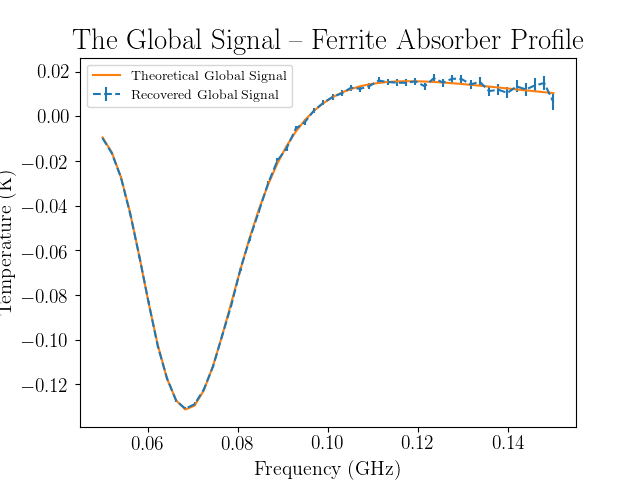
\includegraphics[width=\linewidth]{recovered_signal_same_abs.png}
    \end{center}
    \caption{
        Shown here is the recovered reionization global sky temperature, as 
        measured from a maximally redundant seven element east-west array with 
        a total integrated observation time of five hours, a flat system 
        temperature of $T_{sys} = 300$ K, and pure ferrite absorber baffles. As 
        can be seen, this method of observing the global sky temperature works 
        well, with nearly perfect recovery of the true monopole sky at low 
        frequencies (where our array has the highest sensitivities to the 
        monopole mode) and only small fluctuations (on the order of 3 mK) being 
        introduced at the low-sensitivity high-frequency end of our science 
        band. Although this is a highly idealized case, this is a positive 
        result, indicating that our method of weighting observations can 
        accurately recreate the true 21cm reionization global signal.
    }
    \label{fig:recovered-ferrite}
\end{figure}

Obviously this case is pretty idealized. Our thermal noise is unbiased and 
equal across all frequencies. Our sky is nothing but 21cm reionization monopole 
signal -- there is no galactic synchrotron emission nor spatial structure from 
other sources to account for. Our absorbers have been perfectly understood and 
characterized.

One thing we know about previous 21cm reionization global signal experiments is 
that their downfall comes from the fact that they are delicate. Every component 
of the experiment must be absolutely perfectly understood and calibrated in 
order to be successful, or their signal will be washed away with the 
systematics. So far, this has been an order too tall to be filled.

So what if we introduce a nit? What if something wasn't quite perfect with our 
array? What if, for instance, we didn't quite understand the nature of our 
absorber walls? In particular, what if we miscalibrated the absorptivity of the 
walls as a function of frequency?

In this case, we perform the exact same observation as above. However, where 
the data was actually collected using ferrite absorptive baffles, the 
calibration coefficients were calculated assuming a much simpler absorber 
model: one with a flat 15 dB absorptivity across the whole science band.  
Instead of having a monopole sensitivity like that seen in 
Fig.~\ref{fig:flat-sky-fe-abs-freq}, it looks like 
Fig.~\ref{fig:flat-sky-15dB-abs-freq}. So what happened to our recovered 21cm 
reionization temperature profile?

\begin{figure}
    \begin{center}
    \includegraphics[width=\linewidth]{/home/kara/documents/hyperion/memos/flat_sky_with_15dB_abs_freq_01.png}
    \end{center}
    \caption{
        Shown here is the absolute value of the visibility of a spectrally flat 
        monopole sky versus frequency, for an array with absorptive baffles 
        constructed from a material with a flat absorptivity of 15 dB across 
        the science band. Overall, this case that the lowest absolute 
        sensitivity to the monopole across the band, but it also has the 
        flattest slope for the drop-off in sensitivity, meaning the whole band 
        has relatively higher sensitivity if an observation is integrated just 
        a little while longer.
    }
    \label{fig:flat-sky-15dB-abs-freq}
\end{figure}

Good news! As can be seen in Fig.~\ref{fig:recovered-mismatched}, our recovered 
signal is still largely reflective of the true 21cm reionization global signal.  
The main difference seen comes at the low frequency end, where the recovered 
signal falls just slightly below the true signal up until a frequency of about 
80 MHz. In particular, we see that the main absorption feature of the signal is 
   slightly exaggerated, falling approximately 5 mK below the true signal.

\begin{figure}
    \begin{center}
    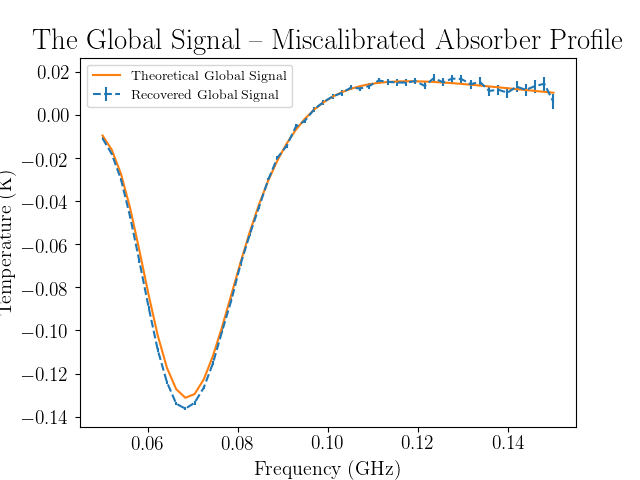
\includegraphics[width=\linewidth]{recovered_signal_diff_abs.png}
    \end{center}
    \caption{
        Shown here is the recovered reionization global sky temperature, as 
        measured from a maximally redundant seven element east-west array with 
        a total integrated observation time of five hours and a flat system 
        temperature of $T_{sys} = 300$ K. In this case, the data was collected 
        from an array using ferrite absorber baffles, but was calibrated 
        assuming the absorber baffles had a flat absorptivity of 15 dB across 
        the science band. As can be seen, even with this intentional gross 
        miscalibration of the system, we are still able to recreate a fairly 
        accurate portrayal of the true 21cm reionization global signal, with 
        the only major difference being a slight 5 mK exaggeration of the depth 
        of the absorption feature. This indicates that our weighting method is 
        robust to an imperfect calibration of the performance of the absorptive 
        baffles -- a promising result for the feasibility of the project.
    }
    \label{fig:recovered-mismatched}
\end{figure}

This is a promising initial result, indicating that the monopole interferometer 
may be more robust to minor calibration issues than its single-element 
counterparts may be. Our recovery isn't perfect in the case of a 
miscalibration, but it's still \emph{good} -- our features are still in the 
right places, the shapes are still there. No false spectral features have been 
introduced, suggesting reionization physics that contradicts the reality of the 
true 21cm reionization global signal.  This reassures us that even as we take 
our system into the backcountry and allow the elements to gently nudge all of 
our perfect lab calibration to the side, we have constructed a system strong 
enough to persist in giving us reasonably accurate answers. This result 
indicates that HYPERION may just have worked.

\chapter{Conclusion}

Within the limited scope of our simulation, particularly our assumptions about 
diffraction and coupling within the element, the ideas behind HYPERION are 
sound.  In this simulation, we manipulated our sensitivity to the global signal 
by imposing a step function onto the beam of our antennas -- thereby converting 
the monopole mode into a series of higher order modes with known scale 
coefficients. We created this step function both by using the pre-existing 
horizon of the Earth to our advantage, and by artificially raising that horizon 
by building absorptive walls around each antenna. Through in-lab testing, we 
have found a promising absorptive material at our low-frequency ranges is 
ferrite, though we are also interested in the idea of a resistive mesh, either 
on its own or layered with the ferrite, depending on its performance. Given 
some knowledge of the  overall performance of an absorber across our science 
band, we are able to simulate a given array design's sensitivity to the 
monopole sky, and thereby generate the scale coefficients for each antenna 
pairing in the array.  Finally, we used these scale coefficients to the 
calibrate and process the observational data, recovering the monopole sky and 
finally getting a glimpse of the global signal.

These results are quite promising, particularly because, as seen in 
Fig.~\ref{fig:recovered-mismatched}, this data processing method is robust 
against at least some types of miscalibration. We were able to completely 
mismatch the true and simulated absorber profiles, and ended up recovering a 
global signal that was only, at most, approximately 5\% different from the true 
input signal. This indicates that, should HYPERION ever be constructed, those 
operating it need not worry about constantly monitoring the state of the 
absorber baffles to get a perfectly accurate measure of their absorptivity for 
each measurement made -- so long as we take care in our initial measurements of 
the absorber baffles, we can be confident that they will remain good enough to 
provide us excellent results in our observations.

Now that we know that these measurements are feasible, and possibly more robust 
to systemic error than our experimental predecessors, we must now continue to 
seek a better understanding of our instrumental design and how to optimize it 
in the face of real observational adversity. So far, we have taken the very 
optimistic view in our simulations that the sky is purely monopole, that there 
are no higher order modes in our signal. In reality, we know that the sky at 
these frequencies is full of galactic structure and extragalactic point 
sources. We simply don't know how well this method of data analysis will work 
when we have a spatially-polluted sky.

The next step to prove the merit of a monopole interferometer would be to input 
a complex sky into the model and see how it behaves. Using accurate global sky 
models alongside our theoretical reionization signal, we can perform the same 
process described in Section~\ref{sec:recovered-signal} and assess our ability 
to recover the reionization global sky, and develop new tools as necessary.

We must also further investigate the realities of the absorbers and how best to 
construct them. To start, we may first assess the viability of the resistive 
mesh concept, testing its absorption across our frequency band and comparing it 
to that of the ferrite tiles. Next, we must begin to explore the full 
electromagnetic system of our antenna-absorber pairs. How does diffraction 
affect our absorber spatial profile? Is there coupling between the absorber and 
the antenna? If so, how does that change our results?

The answers to these questions will determine the long-term viability of this 
method. At present, all we know is that the idea behind a monopole 
interferometer is far less far-fetched than it may have originally seemed. With 
proper calibration and experimental design, it very well could serve a key 
place in the search for understanding the Epoch of Reionization.


\appendix
\chapter{The Flat-Sky Approximation and Its Limitations}
\label{appendix}

In Eq.~\eqref{eq:van-cittert}, we made one implicit assumption -- that we are 
working in only two dimensions. This, of course, is not true. 

In reality, if one is hoping to utilize the nice Fourier nature of the 
brightness and visibility planes, the van Cittert-Zernicke theorem should be 
written in terms of \emph{(u,v,w)} coordinates, rather than just \emph{(u,v)}.  
The full (idealized) measurement equation can thus be written as:

\begin{equation}
    V(u,v,w) = \iint I(l,m) e^{-2\pi i (ul + vm + w\sqrt{1 - l^2 - m^2})} dl dm
    \label{eq:full-measurement}
\end{equation}

The next step is to assume that $l$ and $m$ are small, such that $\sqrt{1 - l^2 
- m^2} \approx 1$, allowing the $e^{-2\pi i w}$ term to be removed from the 
integral by applying the proper phasing to the measured visibility and the 
measurement equation to be simplified to a 2D Fourier transform sampled in the 
\emph{uv}-plane. This procedure is called the \emph{flat-sky approximation}.

This approximation works well for many applications in astronomy, particularly 
in the observation of point sources or small extended sources in the sky (up to 
about $\pm10^\circ$ or so, where $l \equiv \sin\theta \approx \theta$).  
However, as the observed area in the sky gets larger, it becomes impossible to 
apply an absolutely correct phasor to the 2D integral, and the $w$-term instead 
introduces a spatially varying departure from the 2D Fourier transform the 
further from the phase center you are.

So, obviously, in the case where you're trying to use an interferometer to 
observe a global phenomenon (such as the reionization global signal), the flat 
sky approximation simply won't do. In the case that one is attempting to 
perform sky imaging, then care must be taken to navigate the pitfalls of the 
flat-sky approximation, including the use of clunky or expensive algorithms 
such as W-projection. In our case, we are not trying to image the sky at all, 
rather we're just attempting to understand the distribution of power in the 
visibility domain. We can therefore avoid the $(u,v)$ to $(l,m)$ confusion 
entirely and calculate our visibilities directly based on our knowledge of the 
source direction $\mathbf{s}$ and the baseline separation $\mathbf{b}$.


\bibliography{references}{}
\bibliographystyle{apj}

%\printbibliography

\end{document}
